\section{Tutorials 8 (25 IV 2019)}
AFA (alternating finite automaton) $\mathcal{A} = \langle \Gamma, Q, q_I, \lambda, \delta, Win \rangle$\\
$\Gamma$ -- finite\\
$q_I \in Q$\\
$\lambda\ :\ Q \rightarrow [m, n]$\\
$\delta\ :\ Q \times \Gamma \rightarrow B^{+}(Q \times \{+1\})$\\
$w = \Gamma^{\omega}$\\
$G(\mathcal{A}, w):$\\
$V = B^{+}(Q \times \{+1\}) \times pos(\omega)$\\
$v_I = (q_0, 0)$\\
$E:$\\
Eve:\\
$((q+1),n) \rightarrow (\delta(q, w[n]), n+1)$\\
Eve:\\
$(\phi \lor \psi, n) \rightarrow (\phi, n)$\\
$(\phi \lor \psi, n) \rightarrow (\psi, n)$\\
Adam:\\
$(\phi \land \psi, n) \rightarrow (\phi, n)$\\
$(\phi \land \psi, n) \rightarrow (\psi, n)$\\
Eve:\\
$(q_0, 0) \rightarrow (\delta(q_0, w[n]), 1)$\\

\noindent
$A$ accepts $w$ if Eve wins in $G(A, \omega)$\\

\noindent
\textbf{1.} Show that ATA are closed under $\cup, \cap, \lnot$.\\

\noindent
Nonemptiness of an AFA is PSPACE-complete.\\

\noindent
\textbf{Hint for homework}: For EXPTIME-complete, you can use the
following "generic" problem:\\
In: $\mathcal{M}$ -- a (D/N/A) Turing machine, $n \in \mathbb{N}$ in unary\\
Out: Does $M$ accept an empty input using $n$ steps, $n$ memory cell.\\
For deterministic machine it is PTIME-complete (for steps and PSPACE for memory),
for nondeterministic it is (NP-complete for steps and NPSPACE=PSPACE-complete for cells).
For alternating machine it is APSPACE=EXP.

\subsection*{Mean-payoff games}
$G = \langle V, E, \lambda, v_I \rangle$\\
$\lambda:\ E \rightarrow \mathbb{Z}$\\
$p = v_0v_1...v_n...$\\
PG: $\lambda(p \in W$)\\
$\Phi\ :\ plays(G) \rightarrow [0, 1]$\\
$\underset{n \rightarrow \infty}{\lim} \frac{\sum_{i=0}^{n} \lambda(e_n)}{n}$\\

\noindent
\begin{tabular}{| c | c | c |}
    \hline
    & \textbf{MPG} & \textbf{PG}\\
    \hline
    & $\Phi(p)$ & $Parity \ni P$\\
    \hline
    $\delta$ & optimizing strategy & winning strategy\\
    & $\lnot \exists$ & $\exists$\\
    \hline
\end{tabular}\\
$\Phi_{Parity}(p) = \begin{cases}
    1\ \ \ \ \text{parity is even}\\
    0\ \ \ \ \text{if not}
\end{cases}$
\\
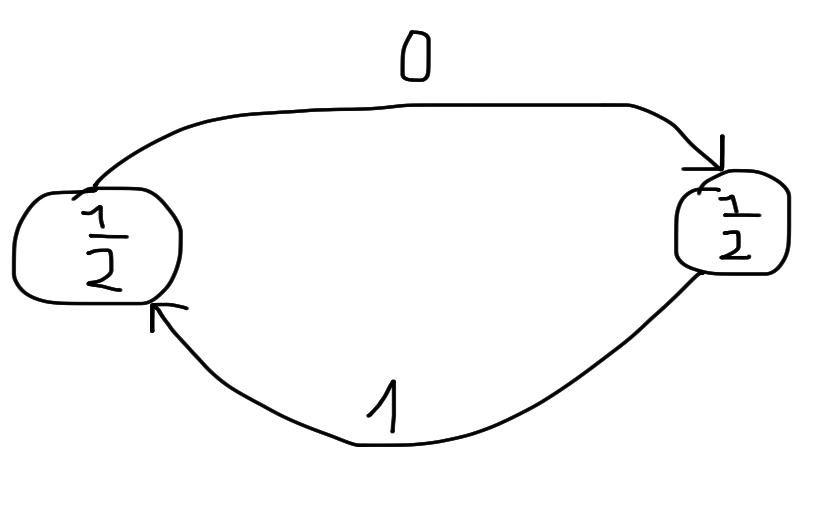
\includegraphics[scale=0.1]{content/graphics/game9.png}\\
$\underline{val} = \underset{\sigma}{sup}\ \underset{\pi}{inf}\ G(\sigma, \pi)$,
$\overline{val} = \underset{\pi}{inf}\ \underset{\sigma}{sup}\ G(\sigma, \pi)$\\


\noindent
a) $\overline{val} \geq \underline{val}$, if = then $G$ is determined\\
b) If $Im(\phi) = \{0, 1\}$ then there is an optimal strategy for one of the players
(or a winning strategy). (Assume $\overline{val} = \underline{val}$)